%%% Thesis Introduction --------------------------------------------------
\chapter{Introduction}
\ifpdf
    \graphicspath{{Introduction/IntroductionFigs/PNG/}{Introduction/IntroductionFigs/PDF/}{Introduction/IntroductionFigs/}}
\else
    \graphicspath{{Introduction/IntroductionFigs/EPS/}{Introduction/IntroductionFigs/}}
\fi

Medical imaging has become a crucial tool in the diagnosis and treatment of various diseases, and the development of new image-processing techniques can help improve the quality and speed of medical imaging, especially MRIs.\\

\nomenclature[zmri]{$MRI$}{Magnetic Resonance Imaging}

Our report is mostly concerned with the use of MRIs, they use magnetic fields and radio waves to create detailed images of the inside of the body, especially useful for soft tissues such as the brain, muscles, and organs. MRIs are non-invasive and do not use ionizing radiation, making them a safer alternative to other imaging technologies such as X-rays or CT scans. However, MRIs can also be expensive and time-consuming to perform, and some patients may not be able to tolerate the confined space of the MRI machine.\\

\begin{figure}[!htbp]
  \begin{center}
    \leavevmode
    \ifpdf
      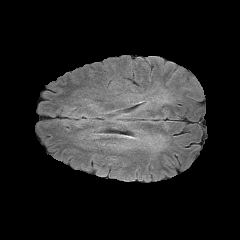
\includegraphics[height=3in]{Introduction/IntroductionFigs/volume_2_slice_88.png}
    \else
      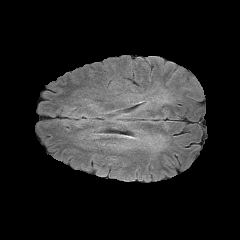
\includegraphics[bb = 92 86 545 742, height=6in]{Introduction/IntroductionFigs/volume_2_slice_88.png}
    \fi
    \caption{A Brain MRI slice \cite{menze2015multimodal, bakas2017advancing, bakas2018identifying}}
    \label{RandomMRI}
  \end{center}
\end{figure}

In recent years, there has been an increased interest in using neural networks to help with this process. We propose two solutions to tackle two of the most important problems concerning MRI.\\

The first problem involves speeding up the process of taking an MRI. To speed up an MRI, we must be able to use the under-sampled MRI that takes lesser time to construct than a fully-sampled MRI output i.e, MRI Reconstruction problem (Section \ref{sec:prob_1} discusses the problem in more detail). Our solution to this problem involves the use of the pre-existing W-Net architecture~\cite{8919674}. The W-Net architecture involves the use of two U-Nets joined together in such a way that the output of one is supplied to the other as input. The first residual U-Net works with the k-space domain MRI data and the second residual U-Net works with the image domain MRI data.\\

Our improvement to this model works with the following idea in mind -- neighbouring MRI slices show very little variations between each other. In our approach, we take only 3 neighbouring slices to show any improvements. The model now takes 3 slices as input and outputs a single close-to-fully-sampled MR image for the middle slice. The neighbours help in providing local information relevant to constructing the middle slice's fully sampled version.\\

The next problem being explored is the well-known problem of super-resolution in MRIs (Section \ref{sec:prob_2} discusses the problem in more detail). In MRIs, however, it's harder to perform super-resolution because we have to ensure that there are minimal artefacts introduced during the super-resolution process. Our approach to solving this problem involves the use of the pre-existing SR3 network \cite{saharia2021image}. Here we don't use MSE (Mean Square Error) as a judgement parameter for the likeness of two images because it doesn't ensure minimisation of artefacts, instead, we propose the use of SSIM (Structural Similarity Index) \cite{1284395} and FID (Fréchet Inception Distance) \cite{fid, mathiasen2021backpropagating}  as both of them promote higher structural similarity. We also want to minimize the noise in the model, a common occurrence in the result of diffusion models such as SR3, so we must also give some weightage to MSE as well.\\

\nomenclature[zssim]{$SSIM$}{Structural Similarity Index}
\nomenclature[zfid]{$FID$}{Fréchet Inception Distance}

Keeping the above in mind, we experimented with variations of the above to study the best use case for MRIs. Our report covers how the difference impacts MRI quality and tries to study the introduction of artefacts.\\

In the report, we aim to show the usefulness of both solutions and how they stand against their baseline counterparts.

%%% ----------------------------------------------------------------------


%%% Local Variables: 
%%% mode: latex
%%% TeX-master: "../thesis"
%%% End: 
